% ============================================================
% SUPPLEMENT 4 (revised, November 2026)
% Hedge-family geometry, logit effects and activity
% The Geometry of SAE Artifacts research program
% ============================================================
\documentclass[11pt,a4paper]{article}

\usepackage[utf8]{inputenc}
\usepackage[T1]{fontenc}
\usepackage{times}
\usepackage{amsmath,amssymb}
\usepackage{graphicx}
\usepackage{booktabs}
\usepackage{hyperref}
\makeatletter\g@addto@macro{\UrlBreaks}{\do\_\do\-\do\.}\makeatother
\usepackage[margin=1in]{geometry}
\usepackage{enumitem}
\usepackage{caption}
\usepackage{natbib}
\usepackage{xcolor}
\usepackage{microtype}
\usepackage{float}
\usepackage{fancyhdr}

\graphicspath{{../figures/supplement4/}}
\hypersetup{colorlinks=true,linkcolor=blue!60!black,citecolor=blue!60!black,urlcolor=blue!60!black}

\setlength{\parskip}{0.4em}
\setlength{\parindent}{0em}

\pagestyle{fancy}
\fancyhf{}
\rhead{\small\textit{Supplement 4 (revised)}}
\lhead{\small\textit{Geometry of SAE Artifacts --- November 2026}}
\cfoot{\thepage}

\newcommand{\cosED}{\cos(E_i, D_i)}

\title{\Large\bfseries Supplement 4 Report (revised): Hedge-Family Geometry,\\
Logit Effects and Activity\\[0.5em]
\large The Geometry of SAE Artifacts Research Program}
\author{\textit{Working report --- November 2026}}
\date{}

\begin{document}
\maketitle
\thispagestyle{fancy}

\begin{abstract}
Supplement~3 identified four strongly anti-aligned features in the Bloom GPT-2 Small layer-8 residual SAE (F19139, F18573, F11969, F20804). The encoders of all four detect the decoder direction of the same feature, F17487, which belongs to a small cluster \{F17487, F21174, F16152\} that we call the parent cluster. This supplement characterises that system using the SAE weights, the GPT-2 unembedding and a snapshot of Neuronpedia metadata. Three results are reported. (1)~In decoder space, F19139 and F11969 are nearly antiparallel to the parent cluster (cosines $-0.48$ to $-0.99$), while F18573 opposes only F17487 and F20804 is close to orthogonal to all of them. (2)~The logit effects of hedge and parent decoders are correspondingly inverted. For F19139 versus F21174, 13 of the top-20 logit tokens appear with opposite sign, and the full logit vectors have Pearson $r = -0.985$. Because logits are a linear function of the decoder vector, this is a restatement of the decoder geometry rather than independent functional evidence. (3)~All seven strongly anti-aligned GPT-2 features queried on Neuronpedia, including features from layers 9 and 10, are dead or nearly dead (activation frequency $\le 3.2\times10^{-7}$). The three parent features are also dead. The only active anti-aligned feature found is Gemma~2B F3378 (layer~1), which is active on 1.7\% of tokens. For the Bloom GPT-2 SAEs, these data favour a dead-feature account (H2) of the most extreme anti-aligned features over an active-hedge account.
\end{abstract}

\medskip\noindent\fbox{\parbox{\dimexpr\linewidth-2\fboxsep-2\fboxrule\relax}{\small
\textbf{Revision note.} This report replaces the March~2026 version of Supplement~4, which has been withdrawn. That version contained a feature-profile table whose values do not match the SAE weights or the Neuronpedia data, decoder cosines attached to the wrong feature pairs, and an analysis of explanations that mixed feature indices across layers. It also labelled four randomly selected layer-8 features (F5977, F22561, F6165, F3696; $\cosED$ at the layer mean) as ``active anti-aligned features''. Its conclusions that anti-alignment is not tied to feature death and that anti-aligned features share no semantic theme rested on those errors. Every number in this version is produced by \nolinkurl{scripts/supplement4_verified_analysis.py}. See \nolinkurl{docs/ERRATA.md} (E3, E6).}}

% ============================================================
\section{Context}

Phase~0 found 35 features in the Bloom GPT-2 Small residual SAEs \citep{bloom2024} with $\cosED < 0$ at or below $\mu - 6\sigma$, all in layers 4--11. Layer~8 contains four of them. Supplement~3 (S3A) applied a bisector test to these four. For each feature $f$ it took $j_{\mathrm{enc}}$, the feature whose decoder is most aligned with $E_f$, and $j_{\mathrm{dec}}$, the feature whose decoder is most opposed to $D_f$. For all four, $j_{\mathrm{enc}}$ is F17487. Three of the four (F19139, F18573, F11969) satisfy the hedge criterion. Their decoders oppose F21174, F17487 and F16152 respectively, which, together with F17487, form the parent cluster.

This supplement asks three questions about that system:
\begin{enumerate}[noitemsep]
  \item What is the full decoder geometry of the hedge and parent features?
  \item Do the opposed decoders produce opposed effects on the output logits?
  \item Are these features active on real text?
\end{enumerate}

% ============================================================
\section{Data and methods}

\paragraph{Weights.} SAE: \texttt{gpt2-small-res-jb}, hook \nolinkurl{blocks.8.hook_resid_pre}, loaded with SAELens. Unembedding: GPT-2 Small $W_U$ as loaded by TransformerLens (layer norm folded, unembedding centred). With this $W_U$, the top-10 positive and negative logit lists of $D_f W_U$ reproduce the lists stored by Neuronpedia for all seven layer-8 features examined (differences are limited to the byte-level display of non-ASCII tokens).

\paragraph{Encoder--decoder cosines.} For every queried feature, $\cosED$ and its deviation from the layer mean (in units of the layer standard deviation) are read from the Phase~1 arrays for the correct model and layer.

\paragraph{Neuronpedia snapshot.} Neuronpedia \citep{neuronpedia} profiles for 26 features (GPT-2 layers 4--11, Gemma~2B layer~1, Llama~3.1~8B layers 0--2) were retrieved on 2026-03-04 by \nolinkurl{scripts/neuronpedia/run_full_analysis.py}. From these profiles we use only the activation frequency (\texttt{frac\_nonzero}, the fraction of tokens in Neuronpedia's activation sample on which the feature is non-zero) and the auto-interpretability explanations. Llama Scope requests returned server errors, so the Llama profiles contain no data. They are reported as missing, not as dead.

\paragraph{Logit inversion.} For a hedge feature $h$ and a parent $p$, let $T^{+}_x$ and $T^{-}_x$ be the 10 tokens with the largest and smallest values of $D_x W_U$. The inversion count is $|T^{+}_h \cap T^{-}_p| + |T^{-}_h \cap T^{+}_p|$, with a maximum of 20. The mean $|\Delta|$ is the mean of $|(D_h W_U)_t + (D_p W_U)_t|$ over inverted tokens $t$; it is small when magnitudes match. We also report the Pearson correlation between the full 50,257-dimensional logit vectors.

% ============================================================
\section{Results}

\subsection{Encoder--decoder alignment of the hedge and parent features}

\begin{table}[H]
\centering
\caption{Layer-8 hedge and parent features. $\sigma$-dev is the deviation of $\cosED$ from the layer-8 mean ($\mu = 0.368$, $\sigma = 0.079$). Activation frequency is from Neuronpedia.}
\label{tab:l8}
\small
\begin{tabular}{@{}llrrrl@{}}
\toprule
Feature & Role & $\cosED$ & $\sigma$-dev & Act.\ frequency & Explanation \\
\midrule
F19139 & anti-aligned, hedge & $-0.526$ & $-11.38$ & $3.2\times10^{-7}$ & legal or criminal actions$^\ast$ \\
F18573 & anti-aligned, hedge & $-0.421$ & $-10.05$ & 0 & --- \\
F11969 & anti-aligned, hedge & $-0.286$ & $-8.33$ & 0 & --- \\
F20804 & anti-aligned, not hedge & $-0.130$ & $-6.35$ & 0 & --- \\
\midrule
F17487 & parent & $+0.822$ & $+5.77$ & 0 & --- \\
F21174 & parent & $+0.605$ & $+3.02$ & 0 & --- \\
F16152 & parent & $+0.483$ & $+1.46$ & 0 & --- \\
\bottomrule
\end{tabular}

\smallskip
{\small $^\ast$Neuronpedia lists a second explanation for F19139: ``overall positive assessments or evaluations''.}
\end{table}

The parents are not anti-aligned. F17487 is in fact one of the most strongly \emph{aligned} features in the layer ($+5.77\sigma$).

\subsection{Decoder geometry}

\begin{figure}[H]
\centering
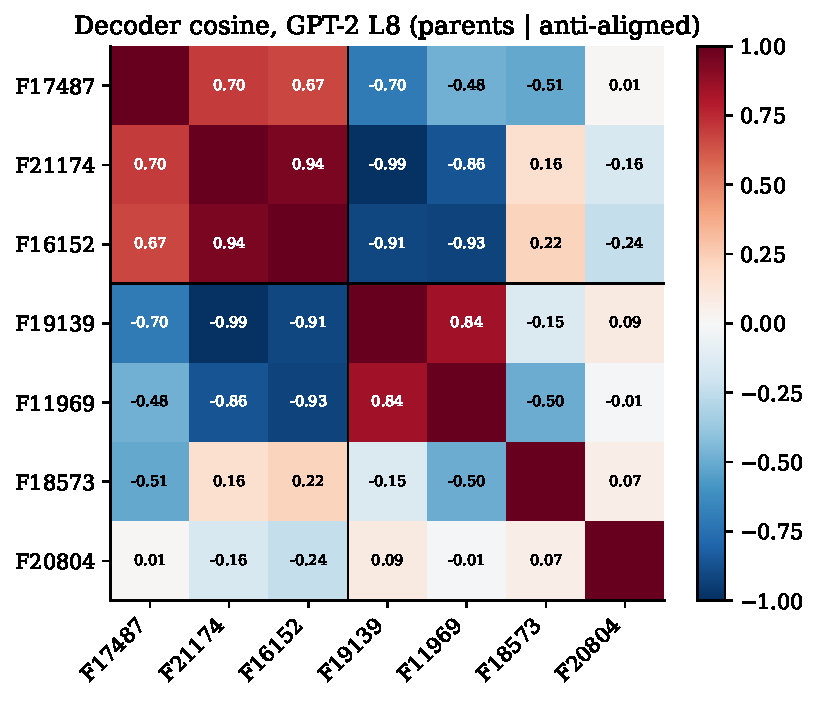
\includegraphics[width=0.62\linewidth]{s4_decoder_cosine_matrix.pdf}
\caption{Pairwise decoder cosines for the parent cluster (top-left block) and the four anti-aligned layer-8 features, computed from $W_{\mathrm{dec}}$.}
\label{fig:deccos}
\end{figure}

Figure~\ref{fig:deccos} shows four structures:
\begin{itemize}[noitemsep]
  \item \textbf{Parent cluster.} F21174--F16152: $0.939$; F17487--F21174: $0.695$; F17487--F16152: $0.671$.
  \item \textbf{Hedge pair.} F19139--F11969: $0.842$. Each member is strongly opposed to every parent ($-0.48$ to $-0.99$). The most opposed pair is F19139--F21174 at $-0.990$, which is nearly antiparallel.
  \item \textbf{F18573.} It opposes F17487 ($-0.511$) but is weakly positive with the other two parents ($+0.16$, $+0.22$) and negative with F11969 ($-0.50$). It passes the encoder-side bisector test, but in decoder space it does not belong to the hedge pair.
  \item \textbf{F20804.} Its decoder cosines with all six other features lie in $[-0.24, +0.09]$, consistent with its failure of the bisector test.
\end{itemize}

\subsection{Logit effects}

\begin{table}[H]
\centering
\caption{Logit effects for hedge--parent pairs. Inversions are counted among the top-10 positive and top-10 negative logit tokens of each decoder (maximum 20).}
\label{tab:logits}
\begin{tabular}{@{}llrrrr@{}}
\toprule
Hedge & Parent & Decoder cosine & Logit-vector $r$ & Inversions (/20) & Mean $|\Delta|$ \\
\midrule
F19139 & F21174 & $-0.990$ & $-0.985$ & 13 & 0.022 \\
F11969 & F16152 & $-0.926$ & $-0.939$ & 10 & 0.070 \\
F11969 & F21174 & $-0.863$ & $-0.872$ & 6 & 0.069 \\
F19139 & F16152 & $-0.908$ & $-0.841$ & 3 & 0.107 \\
F19139 & F17487 & $-0.705$ & $-0.466$ & 1 & 0.181 \\
F11969 & F17487 & $-0.480$ & $-0.388$ & 0 & --- \\
\bottomrule
\end{tabular}
\end{table}

\begin{figure}[H]
\centering
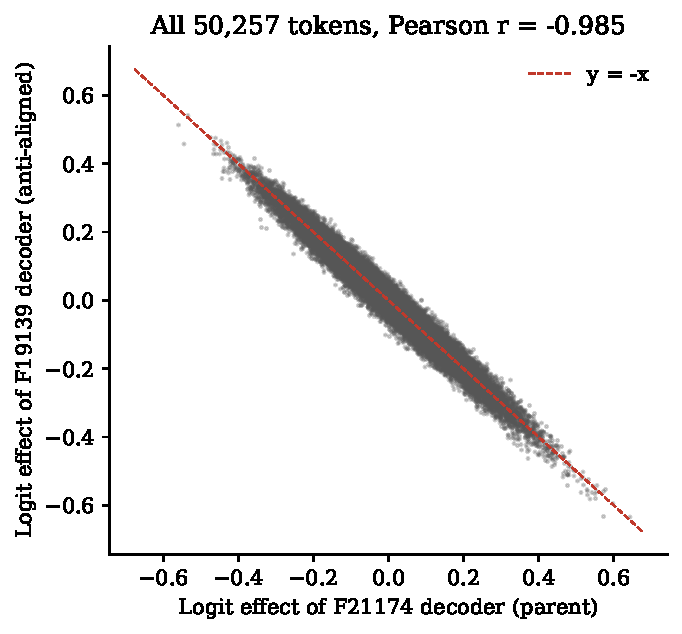
\includegraphics[width=0.5\linewidth]{s4_logit_scatter_F19139_F21174.pdf}
\caption{Logit effect of the F19139 decoder against that of the F21174 decoder for every token in the GPT-2 vocabulary.}
\label{fig:scatter}
\end{figure}

For F19139 and F21174 the inverted tokens include \texttt{SPONSORED}, \texttt{Benz}, \texttt{merce}, \texttt{Logged} and \texttt{onian}, with closely matched magnitudes (mean $|\Delta| = 0.022$). Across the six pairs, the inversion count is rank-correlated with $|\text{decoder cosine}|$ (Spearman $\rho = 0.94$, $n = 6$).

This relationship follows directly from the weights. The logit effect of a decoder is the linear map $D \mapsto D W_U$, so two nearly antiparallel decoders necessarily have nearly antiparallel logit effects. The logit-vector correlation tracks the decoder cosine closely (Table~\ref{tab:logits}); the residual differences reflect the non-isotropy of $W_U$. The logit inversion is therefore a description of the decoder geometry in output-token space. It does not provide independent evidence that the hedge features perform a functional correction during inference, and it cannot, because neither the hedges nor the parents are active (Section~\ref{sec:activity}).

\subsection{Activity}
\label{sec:activity}

\begin{figure}[H]
\centering
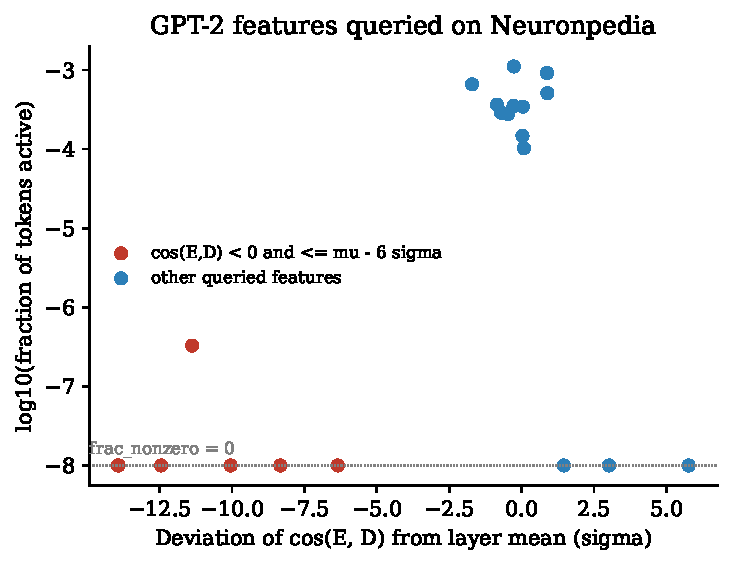
\includegraphics[width=0.62\linewidth]{s4_activity_vs_sigma.pdf}
\caption{Neuronpedia activation frequency against the deviation of $\cosED$ from the layer mean, for the 21 GPT-2 features queried (layers 4--11). Features with frequency zero are drawn on the dotted line.}
\label{fig:activity}
\end{figure}

\begin{itemize}[noitemsep]
  \item \textbf{GPT-2 anti-aligned features.} All seven queried features with $\cosED < 0$ at or below $\mu - 6\sigma$ are dead or nearly dead: the four layer-8 features in Table~\ref{tab:l8}, and the three most extreme features in the whole GPT-2 set (L9/F18298, $-13.94\sigma$; L10/F19679, $-13.92\sigma$; L10/F3268, $-12.45\sigma$). Only F19139 has a non-zero frequency ($3.2\times10^{-7}$, roughly one token in three million).
  \item \textbf{GPT-2 parents.} The three parent features are also dead.
  \item \textbf{Other GPT-2 features.} The remaining 11 queried GPT-2 features have $\cosED$ within $1.71\sigma$ of their layer mean, and all are active (frequency $1.0\times10^{-4}$ to $1.1\times10^{-3}$). Seven of them were queried as controls or random layer-8 samples; four (L4/F18458, L6/F7685, L7/F21750, L11/F4855) had been listed as ``extreme'' in the query script but are not anti-aligned.
  \item \textbf{Gemma~2B F3378} (layer~1, $\cosED = -0.465$, $-8.50\sigma$), the only anti-aligned feature in the Gemma Scope 16k SAEs, is active on 1.7\% of tokens. Its explanation is ``references to software libraries and coding frameworks''.
  \item \textbf{Llama~3.1~8B.} Two queried features are anti-aligned (L1/F27745, L1/F24381), but Neuronpedia returned no data for them. Two others queried as ``extreme'' (L0/F15649, L2/F30420) are not anti-aligned.
\end{itemize}

\subsection{Explanations}

Among the anti-aligned features, only F19139 and Gemma F3378 have auto-interpretability explanations. Dead features have no activating examples to explain. A semantic analysis of anti-aligned features is therefore not possible with these data.

% ============================================================
\section{Discussion}

\paragraph{Geometry.} The decoder geometry agrees with the structure that S3A inferred from the encoders. A tight parent cluster is opposed by two closely related anti-aligned decoders, F19139 and F11969. This is the configuration expected of subtractive correction terms (H1): a feature that fires with a parent concept and removes part of its reconstruction. The near-antipodal pair F19139--F21174 is also reminiscent of the antipodal feature pairs of \citet{elhage2022}. The output-space inversion is analogous in form to copy suppression \citep{mcdougall2023}, but here it arises from weights alone.

\paragraph{Activity.} The hedge mechanism is a statement about what features do when they fire. On Neuronpedia's activation sample, neither the hedges nor their parents fire. For the Bloom GPT-2 SAEs, every strongly anti-aligned feature examined belongs to the dead or near-dead population. This supports H2 (dead-feature decay) as an explanation of the most extreme anti-aligned features, and it raises the possibility that the hedge--parent system is a residue of training dynamics, for example ghost-gradient updates applied to dead features (H4), rather than a mechanism used at inference. The finding is limited to seven features from one SAE family. Whether less extreme anti-aligned features (between $-6\sigma$ and the bulk) are also inactive is open.

\paragraph{Counterexample.} Gemma F3378 shows that anti-alignment can occur in an active feature, in a JumpReLU SAE with per-feature thresholds \citep{lieberum2024}. It is a single feature and was not analysed further.

\paragraph{Relation to absorption.} Feature absorption \citep{chanin2024absorption} produces features whose encoders exclude a sub-case that another feature has absorbed. Anti-aligned hedges could be a related artefact, but establishing this requires co-activation data on live features, which these SAEs do not provide for the hedge family.

% ============================================================
\section{Limitations}

\begin{itemize}[noitemsep]
  \item Activity is taken from Neuronpedia's activation sample. A feature with frequency zero there could fire rarely on other text. Phase~4a (activation frequency on 10M tokens) is required to confirm death.
  \item The analysis covers one SAE family (Bloom GPT-2 Small), one layer for the geometry, and seven anti-aligned features for activity.
  \item Llama Scope features could not be characterised because Neuronpedia returned no data.
\end{itemize}

\section{Implications for later phases}

\begin{enumerate}[noitemsep]
  \item \textbf{Phase~4a first.} Measure activation frequency for all features in the 3-sigma and 6-sigma tails on a fixed corpus. This determines how much of the anti-aligned population is dead.
  \item \textbf{Phase~3.} When retraining SAEs with different seeds, record whether matched anti-aligned features are dead in each run. Train at least one run without ghost gradients to test H4.
  \item \textbf{Hedge interpretation.} Any functional claim about hedges must be tested on active anti-aligned features. Gemma F3378 is currently the only known candidate.
\end{enumerate}

\section*{Reproducibility}

\nolinkurl{scripts/supplement4_verified_analysis.py} produces every table and figure in this report from the SAE weights, the GPT-2 unembedding, the Phase~1 arrays and the Neuronpedia snapshot stored in \nolinkurl{results/supplement4/} (file \nolinkurl{full_analysis_*.json}). It writes \nolinkurl{verified_analysis.json} and \nolinkurl{queried_features.csv} to the same directory.

\bibliographystyle{plainnat}
\bibliography{supplement4}

\end{document}
